
%%% Local Variables:
%%% mode: latex
%%% TeX-master: t
%%% End:

\chapter{实验与分析}
\label{cha:experiments_analysis}
本章节主要介绍在 Spark 集群上进行近似近邻查询算法的实验,主要包括实验环境介绍、实验数据集介绍、实验结果展示以及实验分析。
\section{实验环境}
本次实验中关于 Spark 部分的实验都是在由 4 台机器构成的 Spark on YARN 集群系统上完成的。其中,每台机器配置均相同,配置如下:
\begin{itemize}
\item 操作系统:Red Hat Enterprise Linux Server release 7.0
\item 处理器信息:Intel(R) Xeon(R) CPU E5-2609 0 @ 2.40GHz
\item 核数:8 核
\item 内存大小: 60G
\end{itemize}

关于 MATLAB 部分的实验是在一台单机上完成,配置如下:
\begin{itemize}
\item 操作系统:Windows 8
\item 处理器信息:Intel(R) Core(TM) i3 CPU M 380 @ 2.53GHz
\item 核数:4 核
\item 内存大小: 6G
\end{itemize}
\section{实验数据集}
实验过程中主要使用到了两个数据集,一个是 SIFT1M\footnote{http://corpus-texmex.irisa.fr/},另一个是 CIFAR-10\footnote{http://www.cs.toronto.edu/~kriz/cifar.html}。实验主要对比笔者实现的方法在 Spark 集群系统上与 MATLAB 单机系统上的近似近邻查询的召回率以及相应时间消耗,此外也对比在不同的参数下, Spark 集群系统上的运行结果。
\subsection{SIFT1M}
SIFT1M 是近年来被广泛应用于近似近邻查询方法准确率和召回率的衡量。这个数据集中的数据都是 128 维的 SIFT 特征向量,包含三部分:待索引的原始数据集(base)、训练数据集(learn)、查询数据集(query)。其中待索引的原始数据集合有 $10^6$ 个向量,训练数据集有 $10^5$ 个,查询数据集共有 $10^4$ 个。
\subsection{CIFAR-10}
CIFAR-10 数据集被广泛用于在计算机视觉领域做目标识别、图像分类等任务的。它是从 80 million tiny images\footnote{http://groups.csail.mit.edu/vision/TinyImages/} 数据集中挑选出的一个带标签的子集,由 60000 张 $32\times 32$ 的彩色图像组成。它们被分成 10 类,每个类别有 6000 张图片。10 个类别分别是airplane、automobile、bird、cat、deer、dog、frog、horse、ship、truck。

\begin{figure}[H]
  \centering
  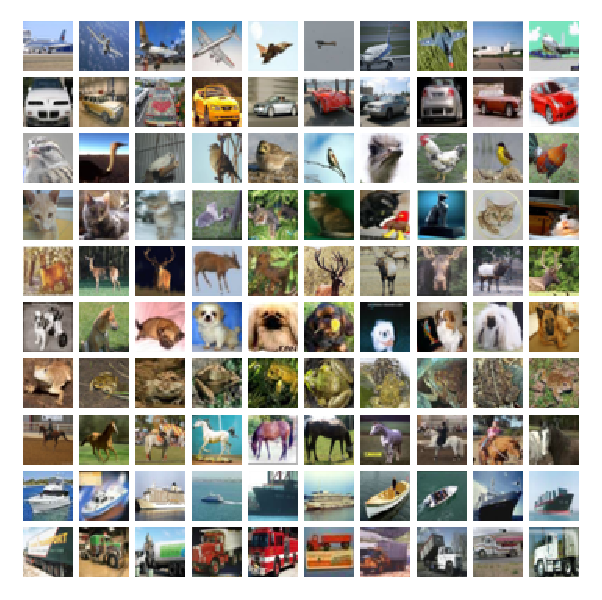
\includegraphics[width=0.7\linewidth]{cifar-10}
  \caption{CIFAR-10 数据集中图片示例}
  \label{fig:cifar-10}
\end{figure}
\section{实验结果与分析}
\subsection{Spark 集群与 MATLAB 对比实验}
本实验室在 SIFT1M 数据上进行,通过比较 Spark 集群上的乘积量化的近似近邻查询方法与 同样方法在 MATLAB 单机上的实验的召回率和时间消耗的对比。

在 Spark 集群系统上的程序参数设置,我们采用 yarn-client 模式在集群上运行程序,设置 executor 的数量为 40,每一个 executor 的内存大小限制为 5G。在对 SIFT1M 数据集近似近邻查询实验中,我们设置子空间切分数量 $m$ 为 8,子空间中的聚类中心数量为 $h$ 为 256,因此总的聚类中心的数量就是 $2^64$,编码字节的大小就是 64 比特。$h$ 取 256 是比较合适的,恰当的子空间聚类中心数量一方面可以使得查找表的大小不会过大,另一方面保证训练和编码的时间也不会太长。在这次实验中,我们采用 recall@$R$ 作为查询效果好坏的衡量标准。SIFT1M 数据中有 $10^4$ 个查询向量,对于一个查询向量,通过整个近似近邻查询计算,我们在原始向量中找到前 100 个近邻向量,并分别取 $R$ 为 1、2、5、10、20、50、100,计算前 $R$ 个向量中出现最近邻向量的次数 $s$,那么衡量标准就可以由公式 recall@$R = s/10^4$ 计算得出。
\begin{table}[htbp]
\noindent\begin{minipage}{0.5\textwidth}
\centering
\caption{Spark 与 MATLAB 上召回率对比}
\label{tab:recall_on_spark_matlab}
\begin{tabular}{ccc}
\toprule[1.5pt]
    & Spark & MATLAB\\
  \hline
  recall@1  &  0.23   & 0.29\\
  recall@2  &  0.33 &   0.40\\
  recall@5  &  0.48 &   0.53\\
  recall@10  & 0.60 &   0.62\\
  recall@20  &  0.72&  0.73\\
  recall@50  &  0.85 &  0.81\\
  recall@100  & 0.92 &  0.88\\
\bottomrule[1.5pt]
    \end{tabular}
\end{minipage}
\begin{minipage}{0.5\textwidth}
\centering
\caption{Spark 与 MATLAB 上时间对比}
\label{tab:time_on_spark_matlab}
\begin{tabular}{ccc}
\toprule[1.5pt]
    & Spark & MATLAB \\
\hline
训练时间(s) & 1193.04 & 1574.09  \\
编码时间(s) & 12.42 & 49.93 \\
单次查询时间(s)& 2.8 & 181.73 \\
\bottomrule[1.5pt]
\end{tabular}
\end{minipage}
\end{table}
表 \ref{tab:recall_on_spark_matlab} 和表 \ref{tab:time_on_spark_matlab} 分别显示的是在 Spark 上与 MATLAB 中的召回率对比以及所用时间对比。仅从表 \ref{tab:recall_on_spark_matlab} 来看,Spark 集群系统上程序的召回率与 MATLAB 单机版本的相差不大。在保证召回率差不多的情况下,我们再看表  \ref{tab:time_on_spark_matlab},从表中我们可以看出在训练阶段的时间消耗上,Spark 比 MATLAB 耗时要少,但是并没有成倍数介绍。在编码阶段时间消耗, Spark 集群上用时仅为 MATLAB 的 $1/4$ 左右。到了查询阶段,单次耗时 MATLAB 是 Spark 集群系统上单次耗时的 $70$ 余倍。
